\section{PHP}

\subsection{Einführung}

\begin{bonus}{Voraussetzungen für PHP}
    Notwendig für einen PHP-Server ist ein installierter \emph{PHP-Interpreter}.

    Typisch für Webententwicklung in PHP ist der \emph{LAMP-Stack}:
    \begin{itemize}
        \item Linux (Betriebssystem)
        \item Apache (HTTP Server)
        \item MySQL (Datenbank)
        \item PHP (Programmiersprache)
    \end{itemize}
\end{bonus}

\begin{defi}{Ablauf einer PHP-Webseite}
    \begin{itemize}
        \item Browser stellt Anfrage an den Server
        \item Dateiendung \texttt{.php} signalisiert dem Server, dass die Datei PHP-Code enthält
        \item PHP-Interpreter interpretiert den Quellcode
        \item Ergebnis wird an den Browser zurückgegeben
    \end{itemize}
\end{defi}

\begin{example}{PHP-Seite}
    Der PHP-Code
    \begin{lstlisting}[language=php,alsolanguage=html]
        <?php
            $titel = "Website des besten Pokemon!";
            $pokemon = "Glumanda"
        ?>

        <!DOCTYPE html>
        <html>
            <head>
                <title> <?php echo $titel; ?> </title>
            </head>
            <body>
                <h1> <?php echo $pokemon; ?> </h1>
            </body>
        </html>
    \end{lstlisting}

    produziert den folgenden HTML-Code:
    \begin{lstlisting}[language=html]
        <!DOCTYPE html>
        <html>
            <head>
                <title>Website des besten Pokemon!</title>
            </head>
            <body>
                <h1>Glumanda</h1>
            </body>
        </html>
    \end{lstlisting}
\end{example}

\subsection{Syntax}

\begin{defi}{Variable (PHP)}
    \emph{Variablen} in PHP werden dargestellt durch \texttt{\$} vor dem Namen.

    Es erfolgt keine explizite Deklaration, also haben Variablen auch keinen festen Typ.

    Nicht initialisierte Variablen haben einen vom Kontext abhängigen Vorgabewert\footnote{z.B. \texttt{false}, \texttt{null}, etc.}.
\end{defi}

\begin{bonus}{Datentypen (PHP)}
    \begin{tabularx}{\textwidth}{|T|l|>{\ttfamily}X|}
        \hline
        \multicolumn{1}{|l|}{Typ} & Beschreibung                & \multicolumn{1}{l|}{Beispiel}               \\
        \hline
        \hline
        boolean                   & Wahrheitswert               & true, false                                 \\
        \hline
        integer                   & Ganzzahl                    & 0, 123, -12, 0xFF                           \\
        \hline
        float / double            & Fließkommazahl              & 3.14, 1.2e5                                 \\
        \hline
        string                    & Zeichenkette                & "Glumanda!"                                 \\
        \hline
        array                     & (assoziatives) Array        & array('key' => 'val'), array(), array(1, 2) \\
        \hline
        object                    & Objekt                      & new Pokemon()                               \\
        \hline
        NULL                      & Variable ohne Wert          & NULL                                        \\
        \hline
        resource                  & Referenz zu einer Ressource & mysql\_connect('localhost', ...)            \\
        \hline
        callable                  & Funktionsreferenz           & function() \{\}                             \\
        \hline
    \end{tabularx}
\end{bonus}

\begin{bonus}{Vergleich (PHP)}
    \emph{Typschwacher} Vergleich mittels \texttt{==}

    {
        \scriptsize
        \centering
        \begin{tabular}{|T||T|T|T|T|T|T|T|T|T|T|T|T|}
            \hline
                  & true          & false         & 1             & 0             & -1            & "1"           & "0"           & "\-1"         & null          & []            & "php"         & " \ "         \\
            \hline
            \hline
            true  & \textbf{true} & false         & \textbf{true} & false         & \textbf{true} & \textbf{true} & false         & \textbf{true} & false         & false         & \textbf{true} & false         \\
            \hline
            false & false         & \textbf{true} & false         & \textbf{true} & false         & false         & \textbf{true} & false         & \textbf{true} & \textbf{true} & false         & \textbf{true} \\
            \hline
            1     & \textbf{true} & false         & \textbf{true} & false         & false         & \textbf{true} & false         & false         & false         & false         & false         & false         \\
            \hline
            0     & false         & \textbf{true} & false         & \textbf{true} & false         & false         & \textbf{true} & false         & \textbf{true} & false         & false         & false         \\
            \hline
            -1    & \textbf{true} & false         & false         & false         & \textbf{true} & false         & false         & \textbf{true} & false         & false         & false         & false         \\
            \hline
            "1"   & \textbf{true} & false         & \textbf{true} & false         & false         & \textbf{true} & false         & false         & false         & false         & false         & false         \\
            \hline
            "0"   & false         & \textbf{true} & false         & \textbf{true} & false         & false         & \textbf{true} & false         & false         & false         & false         & false         \\
            \hline
            "\-1" & \textbf{true} & false         & false         & false         & \textbf{true} & false         & false         & \textbf{true} & false         & false         & false         & false         \\
            \hline
            null  & false         & \textbf{true} & false         & \textbf{true} & false         & false         & false         & false         & \textbf{true} & \textbf{true} & false         & \textbf{true} \\
            \hline
            []    & false         & \textbf{true} & false         & false         & false         & false         & false         & false         & \textbf{true} & \textbf{true} & false         & false         \\
            \hline
            "php" & \textbf{true} & false         & false         & false         & false         & false         & false         & false         & false         & false         & \textbf{true} & false         \\
            \hline
            " \ " & false         & \textbf{true} & false         & false         & false         & false         & false         & false         & \textbf{true} & false         & false         & \textbf{true} \\
            \hline
        \end{tabular}
    }

    \emph{Typstarker} Vergleich mittels \texttt{===}

    {
        \scriptsize
        \centering
        \begin{tabular}{|T||T|T|T|T|T|T|T|T|T|T|T|T|}
            \hline
                  & true          & false         & 1             & 0             & -1            & "1"           & "0"           & "\-1"         & null          & []            & "php"         & " \ "         \\
            \hline
            \hline
            true  & \textbf{true} & false         & false         & false         & false         & false         & false         & false         & false         & false         & false         & false         \\
            \hline
            false & false         & \textbf{true} & false         & false         & false         & false         & false         & false         & false         & false         & false         & false         \\
            \hline
            1     & false         & false         & \textbf{true} & false         & false         & false         & false         & false         & false         & false         & false         & false         \\
            \hline
            0     & false         & false         & false         & \textbf{true} & false         & false         & false         & false         & false         & false         & false         & false         \\
            \hline
            -1    & false         & false         & false         & false         & \textbf{true} & false         & false         & false         & false         & false         & false         & false         \\
            \hline
            "1"   & false         & false         & false         & false         & false         & \textbf{true} & false         & false         & false         & false         & false         & false         \\
            \hline
            "0"   & false         & false         & false         & false         & false         & false         & \textbf{true} & false         & false         & false         & false         & false         \\
            \hline
            "\-1" & false         & false         & false         & false         & false         & false         & false         & \textbf{true} & false         & false         & false         & false         \\
            \hline
            null  & false         & false         & false         & false         & false         & false         & false         & false         & \textbf{true} & false         & false         & false         \\
            \hline
            []    & false         & false         & false         & false         & false         & false         & false         & false         & false         & \textbf{true} & false         & false         \\
            \hline
            "php" & false         & false         & false         & false         & false         & false         & false         & false         & false         & false         & \textbf{true} & false         \\
            \hline
            " \ " & false         & false         & false         & false         & false         & false         & false         & false         & false         & false         & false         & \textbf{true} \\
            \hline
        \end{tabular}
    }

\end{bonus}

\begin{defi}{String (PHP)}
    \emph{Strings} können in PHP mit einfachen Anführungszeichen oder mit doppelten Anführungszeichen erzeugt werden.

    Bei einfachen Anführungszeichen werden Zeichen Steuerzeichen, also z. B. \texttt{\$} oder \texttt{\textbackslash n}, ignoriert.

    Bei doppelten Anführungszeichen werden diese Steuerzeichen interpretiert und Variablen erkannt.
\end{defi}

\begin{example}{String (PHP)}
    Einfache Anführungszeichen:
    \begin{lstlisting}[language=php]
        $pokemon = 'Glumanda';
        $str = 'Das beste Pokemon:\n {$pokemon}'
    \end{lstlisting}
    \texttt{Das beste Pokemon:\textbackslash n \{\$pokemon\}}

    Doppelte Anführungszeichen:
    \begin{lstlisting}[language=php]
        $pokemon = 'Glumanda';
        $str = "Das beste Pokemon:\n {$pokemon}";
    \end{lstlisting}
    \texttt{Das beste Pokemon: \\ Glumanda}

\end{example}

\begin{defi}{Array (PHP)}
    \emph{Arrays} haben in PHP keine feste Größe.

    Assoziative Arrays (vgl. \texttt{HashTable}) sind der Standard für \enquote{eigentliche Arrays}.
\end{defi}

\begin{example}{Array (PHP)}
    Erstellung:
    \begin{lstlisting}[language=php]
        $leer = array();
        $sus = array(591, 'Amoonguss');
        $pokedex = array(
            '001' => 'Bisasam',
            '004' => 'Glumanda',
            '022' => 'Pikachu'
        ); 
    \end{lstlisting}

    Zugriff:
    \begin{lstlisting}[language=php]
        $team = array();
        $team[] = 'Glumanda'; // $team[0] = 'Glumanda'
        $team[] = 'Bisasam'; // $team[1] = 'Bisasam'

        $team[0] = 'Pikachu'; // $team[0] = 'Pikachu'
        $team['Trainer'] = 'Ash' // $team(0 => 'Pikachu', 1 => 'Bisasam', 'Trainer' => 'Ash')
    \end{lstlisting}
\end{example}

\begin{bonus}{foreach-Schleife}
    Da in PHP jedes Array immer assoziativ ist, kann auf folgende zwei Weisen über ein Array iteriert werden:

    \begin{lstlisting}[language=php]
        foreach ($array as $value) {
            // ...
        }
    \end{lstlisting}

    \begin{lstlisting}[language=php]
        foreach ($array as $key => $value) {
            // ...
        }
    \end{lstlisting}
\end{bonus}

\begin{defi}{Einbinden von Dateien (PHP)}
    Dateien können in PHP entweder mithilfe der Keywords \texttt{require} oder \texttt{include} eingebunden werden.

    Unterschiede sind:
    \begin{itemize}
        \item \texttt{require}:
              \begin{itemize}
                  \item \texttt{Fatal Error}, falls Fehler beim Einbinden auftritt (Abbruch der Ausführung)
                  \item oft sinnvoller als \texttt{include}
              \end{itemize}
        \item \texttt{include}:
              \begin{itemize}
                  \item \texttt{Warning}, falls Fehler beim Einbinden auftritt (Ausführung wird fortgesetzt)
                  \item nur bei optionalen Dateien zu verwenden
              \end{itemize}
    \end{itemize}

    Die Keywords \texttt{require\_once} und \texttt{include\_once} funktionieren analog, jedoch werden Dateien auch mehr mehrmaligen Funktionsaufruf nur insgesamt einmal geladen.
\end{defi}

\begin{defi}{Konstante (PHP)}
    In PHP werden \emph{Konstanten} wie folgt definiert:

    \begin{lstlisting}[language=php]
        define(name, value);
    \end{lstlisting}

    Es gilt:
    \begin{itemize}
        \item Der Wert einer globalen Variable kann nicht verändert werden.
        \item Konstanten benötigen kein \texttt{\$}.
        \item Konstanten sind global verfügbar.
        \item Konstanten können nur Strings oder Zahlen sein.
    \end{itemize}
\end{defi}

\begin{defi}{Exception (PHP)}
    \emph{Exceptions} funktionieren wie folgt:

    \begin{lstlisting}[language=php]
        try {
            // ...
        } catch (Exception $e) {
            echo $e->getMessage();
        }
    \end{lstlisting}

    Eigene Exceptions können von \texttt{Exception} abgeleitet werden:

    \begin{lstlisting}[language=php]
        class PokemonException extends Exception {
            // ...
        }

        throw new PokemonException('Glumanda ist zu stark!');
    \end{lstlisting}
\end{defi}

\begin{defi}{Funktion (PHP)}
    In PHP können \emph{Funktionsparameter} explizit per Call-by-Reference übergeben werden:

    \begin{lstlisting}[language=php]
        function add(&$a, &$b) {
            $a += $b;
        }

        $a = 1;
        $b = 2;
        add($a, $b); // $a == 3
    \end{lstlisting}

    Funktionen können eine beliebige Anzahl von Parametern haben:


    \begin{lstlisting}[language=php]
        function f() {
            $num_args = func_num_args(); // Anzahl der Parameter
            $args = func_get_args(); // Array mit Parametern
        }

        add(1, 2, 3);
    \end{lstlisting}
\end{defi}

\begin{defi}{Lambda (PHP)}
    \emph{Lambdas} bzw. \emph{anonyme Funktionen} werden in PHP wie folgt definiert:

    \begin{lstlisting}[language=php]
        $lambda = function($a, $b) {
            return $a + $b;
        };

        echo $lambda(1, 2); // 3
    \end{lstlisting}
\end{defi}

\begin{defi}{Closure (PHP)}
    Ein Lambda wird zum \emph{Closure}, wenn es Zugang zu Variablen bekommt, die normalerweise nicht zur Verfügung stehen würden.

    In PHP gibt es Closures für anonyme und benannte Funktionen.\footnote{Viele Programmiersprachen können nicht beides!}
\end{defi}

\begin{example}{Closure (PHP)}
    \begin{lstlisting}[language=php]
        function pokedex() {
            $dex = array(
                '001' => 'Bisasam',
                '002' => 'Bisaknosp',
                '003' => 'Bisaflor',
                '004' => 'Glumanda',
                // ... 
            )

            // closure 
            return function($id) use ($dex) {
                return $dex[$id];
            };
        }

        $pokemon_getter = pokedex();
        echo $pokemon_getter('004'); // Glumanda
    \end{lstlisting}
\end{example}

\subsection{Objektorientierung}

\begin{bonus}{Zugriff auf Membervariablen}
    In PHP greift man wie folgt auf Member zu:

    \begin{lstlisting}[language=php]
        $this->name     // Innerhalb der Klasse
        $objekt->name   // Ausserhalb der Klasse (falls public)

        self::name      // Zugriff auf static Variable 
        parent::name    // Zugriff auf Elternklasse (static)
    \end{lstlisting}
\end{bonus}

\begin{bonus}{Konstruktor und Destruktor (PHP)}
    Konstruktor:

    \begin{lstlisting}[language=php]
        public function __construct() {
            // ...
        }
    \end{lstlisting}

    Destruktor:

    \begin{lstlisting}[language=php]
        public function __destruct() {
            // ...
        }
    \end{lstlisting}
\end{bonus}

\begin{bonus}{Dateizugriff (PHP)}
    Öffnen einer Datei:
    \begin{lstlisting}[language=php]
        $file = fopen('file.txt', 'r'); // r = read, w = write, a = append, r+ = read/write
    \end{lstlisting}

    Schließen einer Datei:
    \begin{lstlisting}[language=php]
        fclose($file);
    \end{lstlisting}

    Lesen einer Datei bis zu bestimmter Stelle:
    \begin{lstlisting}[language=php]
        $content = fread($file, 100); // liest 100 Bytes
    \end{lstlisting}

    Schreiben in eine Datei:
    \begin{lstlisting}[language=php]
        fwrite($file, 'Hello World!'); // schreibt in die Datei
    \end{lstlisting}

    Existenz einer Datei:
    \begin{lstlisting}[language=php]
        if (file_exists('file.txt')) {
            // ...
        }
    \end{lstlisting}

    Dateigröße:
    \begin{lstlisting}[language=php]
        $size = filesize('file.txt');
    \end{lstlisting}

    Vereinfachte Varianten sind:
    \begin{lstlisting}[language=php]
        $content = file_get_contents('file.txt');       // liest die Datei in einen String
        file_put_contents('file.txt', 'Hello World!');  // schreibt in die Datei,
                                                        // falls sie nicht existiert wird sie erstellt
    \end{lstlisting}

\end{bonus}

\subsection{Dynamische Webseiten}

\begin{bonus}{Aufruf einer statischen Webseite}
    \centering
    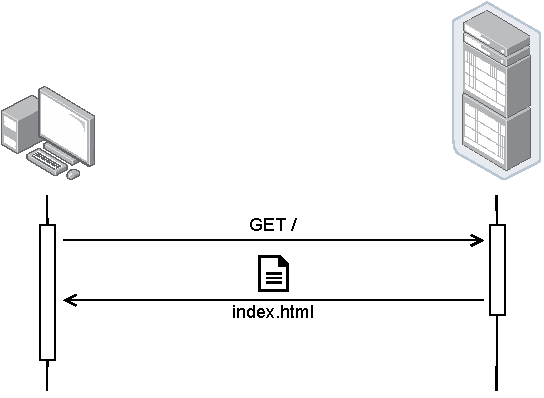
\includegraphics[width=0.7\textwidth]{includes/figures/defi_http.pdf}
\end{bonus}

\begin{bonus}{Aufruf einer dynamischen Webseite}
    \centering
    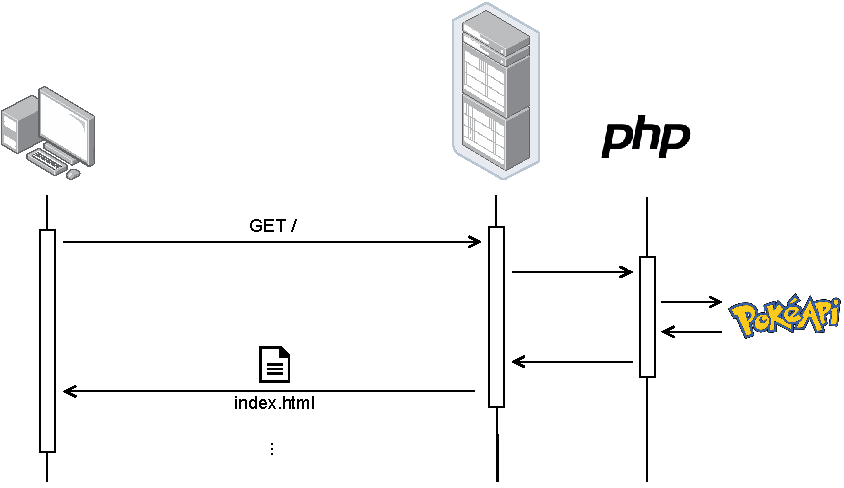
\includegraphics[width=0.8\textwidth]{includes/figures/bonus_dynamisches_php.pdf}
\end{bonus}

\begin{defi}{GET (PHP)}
    Bei \emph{GET}-Methoden werden die Daten über die Adresszeile übertragen.

    Sie sind sind nicht geeignet zur Übertragung großer Datenmengen.

    Parameter werden in PHP im Array \texttt{\$\_GET} gespeichert.
\end{defi}

\begin{example}{GET (PHP)}
    \begin{lstlisting} 
        GET /pokemon^?id=4&name=glumanda^
        HOST: paddel.xyz
    \end{lstlisting}

    Zugriff in PHP:
    \begin{lstlisting}[language=php]
        $_GET['id']; // 4
        $_GET['name']; // glumanda
    \end{lstlisting}
\end{example}

\begin{defi}{POST (PHP)}
    Bei \emph{POST}-Methoden werden die Daten im HTTP-Body übertragen.

    Parameter werden in PHP im Array \texttt{\$\_POST} gespeichert.
\end{defi}

\begin{example}{POST (PHP)}
    \begin{lstlisting} 
        POST /pokemon
        HOST: paddel.xyz

        ^id=4&name=glumanda^
    \end{lstlisting}

    Zugriff in PHP:
    \begin{lstlisting}[language=php]
        $_POST['id']; // 4
        $_POST['name']; // glumanda
    \end{lstlisting}
\end{example}

\begin{defi}{Validierung (PHP)}
    Beschränkungen auf Clientseite können von erfahrenen Nutzenden aktiv umgangen werden, daher ist eine serverseitige Prüfung von Userdaten zwingend erforderlich.

    \emph{Filterfunktionen} vereinfachen in PHP die Validierung von Eingaben.

    Sie liefern \texttt{NULL}, \texttt{false} oder eine je nach Filter gültige Variable zurück.

    \begin{itemize}
        \item \texttt{FILTER\_VALIDATE\_*} validiert Eingaben
        \item \texttt{FILTER\_SANITIZE\_*} korrigiert Eingaben
    \end{itemize}

    Filtern von GET- bzw. POST-Eingaben:
    \begin{lstlisting}[language=php]
        // GET
        if (filter_input(INPUT_GET, 'id', FILTER_VALIDATE_INT)) {
            $name = filter_input(INPUT_GET, 'name', FILTER_SANITIZE_STRING); 
            // ...
        }
    \end{lstlisting}

    \begin{lstlisting}[language=php]
        // POST 
        if (filter_input(INPUT_POST, 'id', FILTER_VALIDATE_INT)) {
            $name = filter_input(INPUT_POST, 'name', FILTER_SANITIZE_STRING); 
            // ...
        }
    \end{lstlisting}

    Filtern von Variablen bzw. Werten:
    \begin{lstlisting}[language=php]
        // Variablen
        $id = filter_var($id, FILTER_VALIDATE_INT);
        $name = filter_var($name, FILTER_SANITIZE_STRING);
    \end{lstlisting}
\end{defi}

\subsection{Datenbanken}

\begin{bonus}{Prepared Statement (PHP)}
    Viele Datenbanken unterstützen beim Nutzen von PDOs\footnote{\emph{PHP Data Objects (PDO)} stellt eine leichte, konsistente Schnittstelle bereit, um mit PHP auf Datenbanken zuzugreifen.} das Konzept der \emph{Prepared Statements}.

    Dabei wird ein SQL-Statement vorbereitet und dann lediglich mit variablen Parametern angepasst.

    Vorteile sind:
    \begin{itemize}
        \item Die Abfrage muss nur einmal geparst werden.
        \item Wenn die Abfrage vorbereitet wird, kann die Datenbank ihre Vorgehensweise zur Ausführung der Abfrage analysieren, kompilieren und optimieren.
        \item Prepared Statements benötigen weniger Ressourcen und laufen deswegen schneller.
        \item Parameter für Prepared Statements müssen nicht maskiert werden. Der Treiber übernimmt das automatisch.
        \item keine SQL-Injection möglich
    \end{itemize}
\end{bonus}

\begin{bonus}{Passwortspeicherung}
    Passwörter sollten nie im Klartext in einer Datenbank gespeichert werden.\footnote{Die Gründe sollten weitestgehend bekannt sein.}

    Hashen eines Passworts in PHP:
    \begin{lstlisting}[language=php]
        $password = 'pok3mon';
        $hash = password_hash($password, PASSWORD_DEFAULT);
    \end{lstlisting}

    Prüfen eines Passworts in PHP:
    \begin{lstlisting}[language=php]
        if (password_verify($password, $hash)) {
            // Passwort ist korrekt
        }
    \end{lstlisting}
\end{bonus}

\subsection{Cookies und Sessions}

\begin{defi}{Cookie (PHP)}
    Der Zustand eines PHP-Skripts geht nach der Ausführung verloren.
    Clients wollen nicht immer alle Daten im Aufruf aktiv mitsenden und der Server möchte auch keine Daten zwischenspeichern.

    Deswegen lässt der Server Daten auf dem Client zwischenspeichern, die der Server nochmal benötigen könnte, damit der Client sie nicht nochmal aktiv senden muss.

    \emph{Cookies} werden z. B. genutzt damit sich der Client einmalig anmelden kann und dann angemeldet bleibt, oder um das Nutzungsverhalten zu analysieren.

    Die Syntax um Cookies zu erstellen sieht wie folgt aus:
    \begin{lstlisting}[language=php]    
        setcookie(
            'name',
            'value',
            [
                'expires' => 'date',
                'path' => 'path',
                'domain' => 'domain',
                'secure' => true,
                'httponly' => true
            ]
        );
    \end{lstlisting}

    Auslesen eines Cookies:
    \begin{lstlisting}[language=php]
        $cookie = $_COOKIE['name'];
    \end{lstlisting}
\end{defi}

\begin{defi}{Session (PHP)}
    Wenn man vertrauliche Daten serverseitig speichern möchte, werden \emph{Sessions} genutzt.

    Die Session-ID wird clientseitig als Cookie gespeichert.

    Starten einer Session:
    \begin{lstlisting}[language=php]
        session_start();
    \end{lstlisting}

    Zugriff auf Session-Variablen:
    \begin{lstlisting}[language=php]
        $_SESSION['lieblings_pokemon'] = 'Glumanda'; // setzt Session-Variable 'lieblings_pokemon'
        echo $_SESSION['lieblings_pokemon'];         // Ausgabe: 'Glumanda'
    \end{lstlisting}

    Beenden einer Session:
    \begin{lstlisting}[language=php]
        session_destroy();
    \end{lstlisting}
\end{defi}